\documentclass[12pt]{article}
\usepackage[utf8]{inputenc}
\usepackage[english]{babel}
\usepackage[normalem]{ulem}
\usepackage{amsmath, amsthm, amssymb, amsfonts}
\usepackage{bm}
\usepackage{enumerate}
\usepackage[margin = 0.75in]{geometry}
\usepackage{graphicx}
\usepackage{wrapfig}
\usepackage{tikz}
\usepackage{hyperref}
\usepackage{color}
\usepackage{xcolor}
\hypersetup{
	colorlinks=true,
	linkcolor=blue,
	filecolor=magenta,      
	urlcolor=cyan,
}
\usepackage{tcolorbox}
\setlength{\parskip}{0.5\baselineskip}%
\setlength{\parindent}{1cm}%


% define new command
\newcommand{\prob}{\mathbb{P}}
\newcommand{\E}{\mathbb{E}}
\newcommand{\Var}{\mathbb{V}}
\newcommand{\Sample}{\mathcal{S}}
\newcommand{\R}{\mathbb{R}}
\newcommand{\C}{\mathbb{C}}
\newcommand{\N}{\mathbb{N}}
\newcommand{\Q}{\mathbb{Q}}
\newcommand{\Z}{\mathbb{Z}}
\newcommand{\contains}{\reflectbox{$\in$}}

\theoremstyle{definition}
\newtheorem{thm}{Theorem}
\newtheorem{lem}{Lemma}
\newtheorem{cor}{Corollary}
\newtheorem{defn}{Definition}
\newtheorem{ex}{Exercise}
\newtheorem{res}{Result}
\newtheorem{prop}{Proposition}



% define theorems and lemmas
\newenvironment{definition}{
\begin{tcolorbox}[colback=green!5!white,colframe=green!75!black, parbox = false]\begin{defn} }{\end{defn}\end{tcolorbox} }

\newenvironment{theorem}{
\begin{tcolorbox}[colback=green!5!white,colframe=green!75!black, parbox = false]\begin{thm} }{\end{thm}\end{tcolorbox} }

\newenvironment{lemma}{
\begin{tcolorbox}[colback=green!5!white,colframe=green!75!black, parbox = false]\begin{lem} }{\end{lem}\end{tcolorbox} }

\newenvironment{result}{
\begin{tcolorbox}[colback=green!5!white,colframe=green!75!black, parbox = false]\begin{res} }{\end{res}\end{tcolorbox} }

\newenvironment{proposition}{
\begin{tcolorbox}[colback=green!5!white,colframe=green!75!black, parbox = false]\begin{prop} }{\end{prop}\end{tcolorbox} }

    
\newenvironment{note}{
\begin{tcolorbox}[colback=blue!5!white,colframe=blue!75!black,title=Note, parbox = false] }{\end{tcolorbox} }

\newenvironment{remark}{
\begin{tcolorbox}[colback=blue!5!white,colframe=blue!75!black,title=Remark, parbox = false] }{\end{tcolorbox} }

\newenvironment{corollary}{
\begin{tcolorbox}[colback=blue!5!white,colframe=blue!75!black, parbox = false]\begin{cor} }{\end{cor}\end{tcolorbox} }
    
\newenvironment{example}{
\begin{tcolorbox}[colback=blue!5!white,colframe=blue!75!black, title = Example, parbox = false] }{\end{tcolorbox} }
    
\newenvironment{exercise}{
\begin{tcolorbox}[colback=red!5!white,colframe=red!75!black, parbox = false]\begin{ex} }{\end{ex}\end{tcolorbox} }


% begin document here
\title{\LARGE \textbf{\textcolor{cyan}{Sample Surveys}}}
\author{M.Stat. $2019-2021$ Batch}
\date{\today}


\begin{document}

\maketitle

\begin{abstract}
    This contains the notes for the course \textit{Sample Surveys}, taught by Dr. Kajal Dihidar for Master of Statistics (M.Stat.) 1st Year batch 2019-20 session. During post midsem of spring $2020$ session, the classes were suspended due to a global pandemic situation created by the breakout of Coronavirus (COVID-19). This notes are intended to cover those lost classes.
\end{abstract}

\pagebreak

\tableofcontents
\pagebreak


\section{Inclusion Probability Proportional to Size Sampling (IPPS)}

\subsection{Introduction to IPPS scheme}

\begin{definition}
    A sampling scheme where the first order inclusion probabilities of all units $\pi_i; i = 1, 2, \dots N$ are proportional to their respective size measure values in auxiliary variable, is called as Inclusion Probability Proportional to size sampling scheme, denoted as \textbf{IPPS} or $\mathbf{\pi}$\textbf{PS}.
\end{definition}

Hence, for this sampling scheme, $\pi_i \propto x_i; \quad i = 1, 2, \dots N$, i.e. $\pi_i = k x_i$, where $k$ is a constant.

As for fixed effective sample size design, (i.e. where $\gamma(s)$ is the number of distinct units in sample $s$, which is equal to $n \quad \forall s \in \S$).

For this, note that, $\sum_{i=1}^N \pi_i = \E(\gamma(s)) = n$. Now, 

\begin{align*}
    & \quad n = k \sum_{i=1}^N x_i\\
    \Rightarrow & \quad n = k X\\
    \Rightarrow & \quad \pi_i = \dfrac{nx_i}{X} = np_i        
\end{align*}

where $p_i = x_i/X$, is the auxiliary size measure probabilities. For IPPS, $\pi_i = n p_i$, for fixed effective sample size designs.

So, Horvitz \& Thompson (1952)'s estimator for population total $Y = \sum_{i=1}^N Y_i$ for a $\pi$PS sampling design is;

$$\hat{Y}_{HT} = \sum_{i \in s} \dfrac{y_i}{\pi_i} = \sum_{i \in s} \dfrac{y_i}{np_i} = \dfrac{1}{n} \sum_{i \in s} \dfrac{y_i}{p_i}$$

which is identical with usual PPSWR population total estimator. However, PPSWR population total estimator contains terms for repeating units as well.

Another important note regarding the $\pi$PS scheme is that $\pi_i = np_i$, but such of the units may have $np_i > 1$. So, we need to be careful about choosing the auxiliary variable, such that it is well related with the main study variable $y$, and also have the all the values $np_i < 1; \quad \forall i = 1, 2, \dots N$.

Now, since the population total estimator formula for both $\pi$PS and PPSWR scheme are same, we may be tempted to deduce that the variances are same for both of them. But we have the following theorem regarding this.

\begin{theorem}
    For a $\pi$PS sampling scheme, if,
    $$\left( 1 - \dfrac{n \pi_{ij}}{(n-1)\pi_i \pi_j} \right) \geq -\dfrac{1}{N-1} $$
    then, we always have;
    $$\Var(\hat{Y}_{PPSWR}) \geq \Var(\hat{Y}_{HT})$$
    which implies that $\pi$PS scheme is always better than PPSWR scheme.
\end{theorem}

\begin{proof}

    Let us denote, 

    \begin{equation}
        \hat{Y}_{PPSWR} = n^{-1} \sum_{i \in s} \dfrac{y_i}{p_i}
        \label{eqn:PPSWR-est}
    \end{equation}
    We know that, 
    \begin{equation}
        \Var(\hat{Y}_{PPSWR}) = n^{-1} \left[ \sum_{i=1}^N \dfrac{Y_i^2}{p_i}  - Y^2 \right]
        \label{eqn:PPSWR-var}
    \end{equation}
    and 
    \begin{equation}
        \Var(\hat{Y}_{HT}) = \sum_{i=1}^N \dfrac{Y_i^2}{\pi_i} + \sum_{i\neq j}^{N} \dfrac{Y_i Y_j}{\pi_i \pi_j} \pi_{ij} - Y^2
        \label{eqn:HT-var}
    \end{equation}
    
    For comparison, we have;
    \begin{align*}
        \Var(\hat{Y}_{PPSWR}) - \Var(\hat{Y}_{HT}) 
        & = Y^2 \left( 1 - \dfrac{1}{n} \right) + \dfrac{1}{n} \sum_{i=1}^N \dfrac{Y_i^2}{p_i} - \sum_{i=1}^N \dfrac{Y_i^2}{\pi_i} - \sum_{i\neq j}^{N} \dfrac{Y_i Y_j}{\pi_i \pi_j} \pi_{ij}\\
        & = Y^2 \dfrac{(n-1)}{n} - \sum_{i\neq j}^{N} \dfrac{Y_i Y_j}{\pi_i \pi_j} \pi_{ij} \qquad \text{since } \pi_i = np_i\\
        & = \dfrac{(n-1)}{n} \left[ \sum_{i=1}^N Y_i^2 + \sum_{i\neq j}^N Y_iY_j \right] - \sum_{i\neq j}^{N} \dfrac{Y_i Y_j}{\pi_i \pi_j} \pi_{ij}\\
        & = \dfrac{(n-1)}{n} \left[ \sum_{i=1}^N Y_i^2 + \sum_{i\neq j}^N Y_iY_j \left( 1 - \dfrac{n \pi_{ij}}{(n-1)\pi_i \pi_j} \right) \right]
    \end{align*}
    Now if, $\left( 1 - \dfrac{n \pi_{ij}}{(n-1)\pi_i \pi_j} \right) \geq -\dfrac{1}{N-1}$, then;
    \begin{align*}
        \Var(\hat{Y}_{PPSWR}) - \Var(\hat{Y}_{HT}) 
        & \geq \dfrac{(n-1)}{n} \left[ \sum_{i=1}^N Y_i^2 - \dfrac{1}{(N-1)} \sum_{i\neq j}^N Y_iY_j  \right]\\
        & = \dfrac{(n-1)}{n(N-1)} \left[ (N-1)\sum_{i=1}^N Y_i^2 - \sum_{i\neq j}^N Y_iY_j \right]
    \end{align*}
    Now, since we can see that,
    \begin{align*}
        \sum_{i\neq j}^N (Y_i - Y_j)^2
        & = \sum_{i\neq j}^N (Y_i^2 + Y_j^2 - 2Y_iY_j)\\
        & = \sum_{i\neq j}^N (Y_i^2 + Y_j^2) - \sum_{i\neq j}^N2Y_iY_j\\
        & = 2(N-1)\sum_{i = 1}^N Y_i^2  - 2\sum_{i\neq j}^N Y_iY_j\\
        & = 2 \left[ (N-1)\sum_{i=1}^N Y_i^2 - \sum_{i\neq j}^N Y_iY_j \right]
    \end{align*}
    Hence we have;
    $$\Var(\hat{Y}_{PPSWR}) - \Var(\hat{Y}_{HT}) \geq \frac{1}{2} \sum_{i\neq j}^N (Y_i - Y_j)^2 \geq 0$$
    
\end{proof}


\begin{note}
    Note that, the condition 
    $$\left( 1 - \dfrac{n \pi_{ij}}{(n-1)\pi_i \pi_j} \right) \geq -\left(\dfrac{1}{N-1}\right) $$ 
    
    implies that, 
    $$\pi_{ij} \leq \dfrac{(n-1)}{n} \dfrac{N}{(N-1)} \pi_i \pi_j $$
    since, $\dfrac{(n-1)}{n} \dfrac{N}{(N-1)} < 1$, as $N >> n$, we have $\pi_{ij} \leq \pi_i \pi_j$ for all $i \neq j$. This condition ensures non-negativity of the variance estimator of HT estimator for fixed effective sample size designs.        
\end{note}


\subsection{Illustration of IPPS scheme}

Durbin (1967) have proposed a procedure of IPPS scheme for $n = 2$. In this procedure, select the first units with probability $p_i$ and the second unit $(j \neq i)$, with probabilities;

$$\prob(j \mid i) = \dfrac{p_j \left[ \dfrac{1}{1-2p_i} + \dfrac{1}{1-2p_j} \right]}{1 + \sum_{i=1}^N \dfrac{p_i}{1 - 2p_i}}$$

for $j \neq i$. In this case, 

\begin{align*}
    \pi_{ij} & = p_i \prob(j \mid i) + p_j \prob(i \mid j)\\
    & = \dfrac{p_ip_j \left[ \dfrac{1}{1-2p_i} + \dfrac{1}{1-2p_j} \right]}{1 + \sum_{i=1}^N \dfrac{p_i}{1 - 2p_i}} +
    \dfrac{p_j p_i \left[ \dfrac{1}{1-2p_j} + \dfrac{1}{1-2p_i} \right]}{1 + \sum_{i=1}^N \dfrac{p_i}{1 - 2p_i}}\\
    & = 2\dfrac{p_i p_j \left[ \dfrac{1}{1-2p_i} + \dfrac{1}{1-2p_j} \right]}{1 + \sum_{i=1}^N \dfrac{p_i}{1 - 2p_i}}
\end{align*}
Now, to compute $\pi_i$, the first order inclusion probabilities, we use;
\begin{align*}
    \pi_i & = \sum_{j \neq i}^N \pi_{ij}\\
    & = \sum_{j \neq i}^N 2\dfrac{p_i p_j \left[ \dfrac{1}{1-2p_i} + \dfrac{1}{1-2p_j} \right]}{1 + \sum_{i=1}^N \dfrac{p_i}{1 - 2p_i}}\\
    & = \dfrac{2 p_i}{1 + \sum_{i=1}^N \dfrac{p_i}{1 - 2p_i}} \left[
        \dfrac{1}{1-2p_i} \sum_{j \neq i}^N p_j + \sum_{j\neq i}^N \dfrac{p_j}{1-2p_j} \right]\\
    & = \dfrac{2 p_i}{1 + \sum_{i=1}^N \dfrac{p_i}{1 - 2p_i}} \left[  \dfrac{1}{1-2p_i} (1-p_i) + \sum_{j\neq i}^N \dfrac{p_j}{1-2p_j}\right]\\
    & = \dfrac{2 p_i}{1 + \sum_{i=1}^N \dfrac{p_i}{1 - 2p_i}} \left[  \dfrac{1}{1-2p_i} (1 - p_i - p_i) + \sum_{j = 1}^N \dfrac{p_j}{1-2p_j} \right]\\
    & = \dfrac{2 p_i}{1 + \sum_{i=1}^N \dfrac{p_i}{1 - 2p_i}} \left[ 1 + \sum_{j = 1}^N \dfrac{p_j}{1-2p_j} \right]\\
    & = 2p_i
\end{align*}


Therefore, $\pi_i = np_i$, where $n = 2$ here. Hence, it is IPPS scheme. For $n \geq 2$, the IPPS scheme will be discussed in next section.

\subsection{IPPS Scheme for $n>2$}
Sampford (1967) has given a IPPS scheme with normed size measure $p_i$ attached to the $i^{th}$ unit so that the first order inclusion probability for the $i^{th}$ unit becomes $\pi_i = np_i$. This sampling design is as follows:

On the first draw the $i^{th}$ unit is selected with probability $p_i(1)=p_i$. Then the remaining $(n-1)$ units are drawn with replacement from the entire population with probability proportional to $\lambda_i = \dfrac{p_i}{1-np_i}$ attached with the $i^{th}$ unit i.e, the probability of selecting $i^{th}$ unit at $k^{th}$ draw is,
$$p_i(k)=\dfrac{\lambda_i}{\displaystyle \sum_{j=1}^N \lambda_j}, \quad k=2,3,\cdots,n.$$
The selected units are accepted as a sample if all the $n$ units happen to be different, otherwise the entire selection is discarded and this process is repeated until aset of distinct units is obtained.


Sampford (1967) has shown that the inclusion probability for the selection of $i^{th}$ unit is $\pi_i=np_i$ and $\pi_i\pi_j-\pi_{ij}\geq 0$. (Not shown here).

The expression for the second order inclusion probabilities are not simple. However, approximate expression of $\pi_{ij}$ correct upto $O(N^{-4})$, derived by Asok and Sukhatme (1976) for $n\geq 3$ is,
\begin{align*}
    \pi_{ij} & =n(n-1)p_ip_j\left[1+\left(p_i+p_j-\sum_{j=1}^N p_j^2\right) \right. \\
    & + \left\{2(p_i^2+p_j^2)-2\sum_{j=1}^N p_j^3 - (n-2)p_i p_j \right. \\ 
    & \left. \left.  +(n-3)(p_i+p_j)\sum_{j=1}^N p_j^2-(n-3)\left(\sum_{j=1}^N p_j^2\right)^2 \right\}
    \right]
\end{align*}
Once these are obtained, HT estimator for population total $Y=\sum_{i=1}^N Y_i$ and corresponding variance estimator can be employed.\\
(Proofs are not shown here. Interested students may see the concerned reference.)

\subsection{Another Illustration of IPPS Scheme}

Let us consider Lahiri, Midzuno and Sen (1952)'s scheme of unequal probability sampling with the normed size measure value $p_i=\dfrac{x_i}{X}$ attached with unit $i, \quad i=1,2,\cdots ,N$.

In this scheme, the first unit is drawn by PPS with $p_i$ values as normed size measures. Then from the remaining $(N-1)$ population units, $(n-1)$ units are selected by SRSWOR. So, in this scheme,
\begin{align*}
    \pi_i & = p_i +(1-p_i)\cdot \dfrac{{N-2 \choose n-2}}{{N-1 \choose n-1}}\\
    & = p_i + (1-p_i)\cdot \dfrac{n-1}{N-1}\\
    & = p_i \left(1-\dfrac{n-1}{N-1}\right)+\dfrac{n-1}{N-1}\\
    \implies \pi_i & = p_i\cdot\dfrac{N-n}{N-1}+\dfrac{n-1}{N-1}\\
    \implies \pi_i & \text{is not proportional to} p_i.
\end{align*}
In general, this scheme is \textbf{NOT} an IPPS scheme.

To modify this scheme to make an IPPS scheme, let us consider a new selection probability as $p_i^*$. $p_i^*$ values can be obtained in the following way:

According to $p_i^*$ selection probability of the unit $i$, 
\begin{align*}
    \pi_i & = p_i^* +(1-p_i^*)\cdot \dfrac{{N-2 \choose n-2}}{{N-1 \choose n-1}}\\
    & = p_i^* + (1-p_i^*)\cdot \dfrac{n-1}{N-1}\\
    & = p_i^*\cdot\dfrac{N-n}{N-1}+\dfrac{n-1}{N-1}\\
\end{align*}
To make this scheme an inclusion probability proportional to normed size measure value $p_i$, we equate,
$$p_i^*\cdot\dfrac{N-n}{N-1}+\dfrac{n-1}{N-1}=np_i$$
This gives,
\begin{align*}
    p_i^* & = \left(np_i-\dfrac{n-1}{N-1} \right)\times\dfrac{N-1}{N-n}\\
    \implies p_i^*  & =\dfrac{n(N-1)}{N-n}\cdot p_i - \dfrac{n-1}{N-n}
\end{align*}
So, considering $p_i^*$ as the selection probabilities, LMS scheme can be connected to an IPPS scheme. Then $\pi_i=np_i \quad \forall i=1,2,\cdots , N$. And,
$$\pi_{ij}=p_i^*\cdot \dfrac{{N-2 \choose n-2}}{{N-1 \choose n-1}}+p_j^*\cdot \dfrac{{N-2 \choose n-2}}{{N-1 \choose n-1}}+(1-p_i^*-p_j^*)\cdot \dfrac{{N-3 \choose n-3}}{{N-1 \choose n-1}} \quad \forall i\neq j \in \mathbf{V} = \{1,2,\cdots,N\}.$$
For this scheme, $\pi_i\pi_j>\pi_{ij}\quad\forall i\neq j \in \mathbf{V}$.

\begin{exercise}
The following figures relate to a group of $15$ households.
    \begin{center}
    \begin{tabular}{|l|l|l|}
    \hline
    Serial No. & HH Size & Expenditure last month (Rs.)  \\ \hline
        1 & 8 & 5470.35 \\ \hline
        2 & 6 & 2716.80 \\ \hline
        3& 5& 1873.75 \\ \hline
        4& 4& 1693.20\\ \hline
        5& 3& 1393.55\\ \hline
        6& 6& 2398.74 \\ \hline
        7& 2& 3153.35\\ \hline
        8& 5& 2708.75\\ \hline
        9& 7& 2873.60\\ \hline
        10& 6& 3775.80\\ \hline
        11& 8& 5027.25\\ \hline
        12& 3& 1175.28\\ \hline
        13& 4& 2952.15\\ \hline
        14& 2& 1032.27\\ \hline
        15& 2& 2075.41\\ \hline
    \end{tabular}
    \end{center}
    \begin{itemize}
        \item[(i)] Consider the above data as a population data. Consider estimates of average last month's h.h. expenditure in this area based on a IPPS sample survey of size $n=2$ h.h.s. with h.h. size as size measure. \\
        Use Durbin (1967)'s IPPS scheme and give your estimate, standard error estimate, c.V. estimate, $95\%$ C.I. of $\Bar{Y}$.
        \item[(ii)] Do the same exercise of IPPS scheme using $n=6$ h.h.s. and modified Lahiri-Midzuno-Sen (1952)'s scheme.
    \end{itemize}
\end{exercise}


% class 3
\section{Double Sampling or Two Phase Sampling}

In many frequently occurred problems of survey sampling situations, a survey population may be composed of a number of its non-overlapping components distinguishable in terms of the values of a variable defined on it taken across disjoint ranges. But the individuals taking values within the respective intervals may not be identifiable and moreover how many of them take values within the disjoint intervals may or may not be known either to begin with. Thus, we may decide on \textbf{stratification} as an efficient estimation procedure, but may not be in a position to implement it well to a desired extent possible. Double Sampling is a way to get rid of this problem.

Again in another practical situation, we know that to employ a ratio estimator or its allied regression estimator for a survey population total, the population total of the considered auxiliary variable needs to be known. But, in many practical cases, this may not be known. Double sampling helps us in such situation.

Again, in case no data can be gathered from some of the sampled units, double sampling provides a clue to handle such non-response situation.

To motivate you with another example, if a survey is to be repeated on two or more occasions, not widely apart spatially or temporally, estimation for the current one may be improved using the past data, applying principles of double sampling in a suitably modified way.

Essentially the double sampling procedure supposes taking on an initial sampling, use it for gathering data on the variable of interest itself and / or on one or more related variables and utilize the accumulated material in developing an improved survey and estimation procedure for the parameter of ultimate interest.

Let us discuss below in detail some application of double sampling. Double Sampling in non-response situation in survey sampling is discussed previously (during B3 course), based on Hansen and Hurwitz's work. Now we discuss the use of double sampling in stratified random sampling.


\subsection{Double Sampling for Stratification}

Suppose we define the $h$-th stratum of a sruvey population of $N$ units, as the set of units bearing $y$-values in the range $(a_{h-1}, a_h)$ for $h = 1, 2, \dots H$. With this stipulated range specified but not completely known in the sense that which units and how many of them have $y$-values within these respective ranges.

Let $W_h = \dfrac{N_h}{N}$, for $h = 1, 2, \dots H$, be the unknown population stratum strengths, where $N_h$ is the unknown number of units in $h$-th stratum.

In such a situation, though the stratified random sampling is the best decided scheme, but it is not possible to start with. In order to get rid of this problem, the following may be tried.

Let a SRSWOR of $n_1$ units be taken and $y$-values of these selected units are collected. Based on the collected $y$-values, we distribute $n_1$ sampled units to $H$ predefined strata.

Let $n_{1h}$ be the number of units falling in the $h$-th range $(a_{h-1}, a_h)$. Let independently across $H$ strata, for $h = 1, 2, \dots H$, SRSWOR of sizes $n_{2h}$ be drawn out of $n_{1h}$ units. And then, based on these $n_{2h}$ sampled units, the data values $\bar{y}_{2h}$ be the sample mean for $h$-th stratum of $y$-values.

Letting, $w_{1h} = \dfrac{n_{1h}}{n_1}$. Let us denote $\E_1, \E_2, \E$ and $\Var_1, \Var_2, \Var$ as the expectation and variance operators with respect to sample selection initially, stratified sampling of $n_{2h}$ units out of them realized sets of $n_{1h}$ units for $h = 1, 2, \dots H$ and the overall sampling procedure.

Let, $\bar{y}_{st} = \sum_{h = 1}^{H}w_h \bar{y}_{2h}$.

\begin{theorem}
    $\bar{y}_{st}$ is an unbiased estimator of $\bar{Y}$.
\end{theorem}

\begin{proof}

We have,
\begin{align*}
   \E_2(\bar{y}_{2h}) & = \bar{y}_{1h} = \dfrac{1}{n_{1h}} \sum_{i = 1}^{n_{1h}} y_{hi}\\
   & \\
   \E_1(w_h) & = \E_1\left( \dfrac{n_{1h}}{n_1} \right) = \dfrac{N_h}{N} = W_h\\
\end{align*}

Therefore,
\begin{align*}
    \E(\bar{y}_{st}) & = \E_1 \E_2 \left( \sum_{h = 1}^{H}w_h \bar{y}_{2h} \right)\\
    & = \E_1 \left( \sum_{h = 1}^{H}w_h \bar{y}_{1h} \right)\\
    & = \E_1 \left( \sum_{h = 1}^{H} \dfrac{n_{1h}}{n_1} \dfrac{1}{n_{1h}} \sum_{i = 1}^{n_{1h}} y_{hi} \right)\\
    & = \E_1 \left( \dfrac{1}{n_1} \sum_{h = 1}^{H} \sum_{i = 1}^{n_{1h}} y_{hi} \right)\\
    & = \E_1(\bar{y}_1) = \bar{Y}
\end{align*}

where the last equality follows from the fact that $\bar{y}_1$ is the sample mean of the initial SRSWOR sample of size $n_1$, which is unbiased for population mean.

\end{proof}

Regarding the variance of the estimator, we have the following theorem.

\begin{theorem}
    $$\Var(\bar{y}_{st}) = \left( \dfrac{1}{n_1} - \dfrac{1}{N} \right)S^2 + \dfrac{1}{n_1} \sum_{h=1}^{H} \left(\dfrac{1}{\gamma_h} - 1\right) W_h S_h^2$$
    where,
    \begin{align*}
        S^2 & = \dfrac{1}{(N-1)} \sum_{i = 1}^{N} \left( Y_i - \bar{Y} \right)^2 = \text{ Population variance of } y\\
        \gamma_h & = \dfrac{n_{2h}}{n_{1h}} = \text{ Fixed sampling fraction at 2nd phase for } h \text{-th stratum}\\
        S_h^2 & = \dfrac{1}{(N_h-1)} \sum_{i = 1}^{N_h} \left( Y_{hi} - \bar{Y}_h \right)^2 = = \text{ Population variance for } h \text{-th stratum}\\
    \end{align*}
\end{theorem}


\begin{proof}

Note that, $\E_2(\bar{y}_{st}) = \bar{y}_1$, which is SRSWOR sample mean. 

Hence, $\Var_1\E_2(\bar{y}_{st}) = \Var_1\left( \bar{y}_1 \right) = \left( \dfrac{1}{n_1} - \dfrac{1}{N}\right)S^2$.

Now, 
\begin{align*}
    \Var_2\left( \bar{y}_{st} \right) & = \Var_2 \left( \sum_{h = 1}^{H}w_h \bar{y}_{2h} \right)\\
    & = \sum_{h = 1}^{H} w_h^2 \Var_2(\bar{y}_{2h})\\
    & = \sum_{h = 1}^{H} \dfrac{n_{1h}^2}{n_1^2} \left( \dfrac{1}{n_{2h}} - \dfrac{1}{n_{1h}} \right) \dfrac{1}{n_{2h} - 1} \sum_{i = 1}^{n_{1h}} \left(y_{hi} - \bar{y}_{1h}\right)^2\\
    & = \sum_{h = 1}^{H} \dfrac{n_{1h}^2}{n_1^2} \left( \dfrac{1}{n_{2h}} - \dfrac{1}{n_{1h}} \right) s_{1h}^2 \text{, where } s_{1h}^2 \text{ is the quantity it is replacing}\\
    & = \sum_{h = 1}^{H} \dfrac{n_{1h}}{n_1} \left( \dfrac{1}{n_{2h} / n_{1h}} - 1 \right) s_{1h}^2\\
    & = \sum_{h = 1}^{H} \dfrac{n_{1h}}{n_1} \left( \dfrac{1}{\gamma_h} - 1 \right) s_{1h}^2\\
\end{align*}

Now let $\E_{1c}$ denotes the expectation conditioned on the fixed configuration of $\mathbf{n}_1 = \left(n_{11}, n_{12}, \dots n_{1H}\right)$, and $\E_{1u}$ denotes the expectation operator over the variability inherent in the sampling of the 1st phase.

So, 

$$\E_{1c}(s_{1h}^2) = \E_{1c}\left( \dfrac{1}{n_{2h} - 1} \sum_{i = 1}^{n_{1h}} \left(y_{hi} - \bar{y}_{1h}\right)^2 \mid \mathbf{n}_1 \right) = S_h^2$$

Also, $\E_{1u}(w_h) = \E_{1u}\left( \dfrac{n_{1h}}{n_1} \right) = \dfrac{N_h}{N} = W_h$.

So, $\E_1(w_h s_{1h}^2) = W_hS_h^2$. Hence,

$$\Var(\bar{y}_{st}) = \E_1\Var_2(\bar{y}_{st}) + \E_2\Var_1(\bar{y}_{st})$$, which reduces to the above quantity, i.e.

$$\Var(\bar{y}_{st}) = \left( \dfrac{1}{n_1} - \dfrac{1}{N} \right)S^2 + \dfrac{1}{n_1} \sum_{h=1}^{H} \left(\dfrac{1}{\gamma_h} - 1\right) W_h S_h^2$$

\end{proof}


\begin{note}
Estimations of $\Var(\bar{y}_{st})$ is quite complicated and will be discussed in higher class. \textbf{Seriously?? Higher Class??}

Chaudhuri (2010) has given an unbiased estimator for $\Var(\bar{y}_{st})$ as follows:

\begin{multline*}
    \hat{\Var}(\bar{y}_{st}) = \dfrac{ \left( \dfrac{1}{n_1} - \dfrac{1}{N} \right) \dfrac{N}{N-1} }{1 - \left( \dfrac{1}{n_1} - \dfrac{1}{N} \right) \dfrac{N}{N-1}} \left[
    \left\{
    \sum_{h = 1}^{H} w_h \left( \bar{y}_{2h}^2 - \dfrac{1}{n_{2h}} \right)\left( \dfrac{1}{\gamma_h} \right)s_h^2 \right\} - \bar{y}_{st}^2 \right]\\
    + \dfrac{1}{n_1} \sum_{h = 1}^{H} \left( \dfrac{1}{\gamma_h} - 1 \right)w_h s_h^2
\end{multline*}

\begin{exercise}
You may try to compute its expectation and show that it is indeed an unbiased estimator of the variance.
\end{exercise}
\end{note}

Now, suppose that although the units are not properly assignable to the respective strata as their $y$-values are unknown to begin with, how many units $N_h$ belong to the respective $h$-th stratum is known somehow to a reliable extent. In such a situation, let a SRSWOR of size $n$ be drawn from the population of $N$ units. Next, to implement the survey, the sampled units are assigned to the respective ranges $(a_{h-1}, a_h)$ in respect of their $y$-values obtained after the survey. Since, $W_h = \dfrac{N_h}{N}$ are known, an unbiased estimator of $\bar{Y} = \sum_{h = 1}W_h \bar{Y}_h$ can be taken as;

$$\bar{y'}_{st} = \sum_{h = 1}^{H} W_h \bar{y}_h \dfrac{I_h}{\E(I_h)}$$

where $\bar{y}_h$ is the mean of the $y$-values for the $n_h$ units that are observed to fall in the $h$-th stratum. Note that, for some of the strata, $n_h$ can be zero. For that stratum, we have $\bar{y}_h = 0$. Also, 

$$I_h = \begin{cases}
1 & \text{ if the h-th stratum has } n_h > 0\\
0 & \text{ otherwise}
\end{cases}$$

So, 

$$\E(I_h) = \prob(I_h = 1) = \prob(n_h > 0) = 1 - \prob(n_h = 0) = 1 - \dfrac{\binom{N - N_h}{n}}{\binom{N}{n}}$$

\begin{definition}
    Such strata that are formed after taking an initial sample and then distributing the sampled units based on their collected $y$-values, are called \textbf{Post Stratification}.
\end{definition}

% class 4

\section{Randomized Response}

Many times surveys relate to sensitive and stigmatizing issues. For example, a social survey may have the objective to obtain an idea about the percentage of people in a given community having undesirable traits, like uncontrolled alcoholism, habitual drunken driving, underpayment of income taxes etc. Many other examples may be experiences i  induced abortion, HIV positivity and suffering from AIDS, gambling habits etc. as possible qualitative features that people are inclined to hide. Similarly, amounts of income tax evaded, money lost or gained in gambling, numbers of induced abortions experienced, amounts spent on alcoholism during last week etc. are several instances of quantitative variables which are often socially felt to be stigmatizing. In such situations, an investigator often feels hesitation to directly ask the questions and also after asking such questions the answers obtained are likely to be unreliable.

In order to get rid of these difficulties in such surveys, a special technique called \textbf{Randomized Response Technique} was introduced by Warner (1965, JASA). 

In this technique, for every person sampled, no matter how, is offered a box having a large number of identical cards differing only in the proportions $p$ of them carrying the mark $A$(meaning sensitive characteristics) and $(1-p)$ where $0< p \neq \frac{1}{2} < 1$ of them bearing the mark $A^c$. 

\begin{wrapfigure}{r}{7.5cm}\label{SS1}
\centering
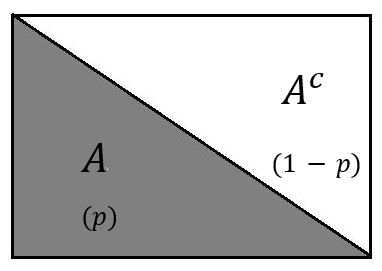
\includegraphics[width=5.5cm]{SS figures/SS1.JPG}
\caption{Box (called \textbf{Randomized Response Device (RRD).}}\label{SS1}
\end{wrapfigure}
Every respondent bearing either the stigmatizing characteristics $A$ or its complement $A^c$ is requested by the investigator to randomly draw one card from the box and respond as,
\begin{itemize}
    \item \textbf{``YES"} if his own characteristics matches with the mark on the card drawn by him.
    \item otherwise \textbf{``NO"} if his own characteristics does not match with the mark on the card drawn by him.
\end{itemize}
 
The investigator does not observe what card is drawn by the respondent, he just collects the answer ``YES" or ``NO" from the respondent, this way the respondent's privacy is protected.

Warner (1965) considered the sampling scheme of selecting the respondents as \textbf{SRSWR}.

Let us denote the population proportion of persons having sensitive attribute $A$ as $\theta_A$. Our objective is to estimate $\theta_A$ by Warner (1965)'s model. Out of the $n$ sampled respondents selected by SRSWR, let $n_1$ respondents reports ``YES".

Now the probability of obtaining ``YES", say $\lambda$ can be written as,
\begin{align*}
    \lambda & = p \theta_A +(1-p)(1-\theta_A)\\
    & = p\theta_A + 1- p - \theta_A +p \theta_A \\
    & = (1-p) + (2p-1)\theta_A \\
    \implies \theta_A & = \dfrac{\lambda -(1-p)}{2p-1} \quad \text{provided} \quad p\neq \frac{1}{2}
\end{align*}
Now $\lambda=$ probability of ``YES" responses can be estimated by, $\hat{\lambda}=\dfrac{n_1}{n}$. Hence an unbiased estimator of $\theta_A$ is,
$$\hat{\theta}_A=\dfrac{\hat{\lambda} -(1-p)}{2p-1}=\dfrac{\dfrac{n_1}{n} -(1-p)}{2p-1} \quad \text{provided} \quad p\neq \frac{1}{2}.$$
\begin{note}
The RRD making $p$ is taken different from $\dfrac{1}{2}$ because of having a valid estimator formula for $\theta_A$.
\end{note}
The variance of this estimator $\hat{\theta}_A$ is,
$$\Var(\hat{\theta}_A)=\dfrac{\Var(\hat{\lambda})}{(2p-1)^2}=\dfrac{\lambda(1-\lambda)}{n(2p-1)^2},\quad \text{because}\quad \Var(\hat{\lambda})=\dfrac{\lambda(1-\lambda)}{n}\quad \text{for SRSWR.}$$
Putting $\lambda= p\theta_A +(1-p)(1-\theta_A)$, we have,
$$\Var(\hat{\theta}_A)=\dfrac{\theta_A(1-\theta_A)}{n}+\dfrac{p(1-p)}{n(2p-1)^2}.$$
To estimate $\Var(\hat{\theta}_A)$ :---
$$\hat{\Var}(\hat{\theta}_A)=\dfrac{\hat{\Var}(\hat{\lambda})}{(2p-1)^2}=\dfrac{\hat{\lambda}(1-\hat{\lambda})}{(n-1)(2p-1)^2}.$$
\begin{note}
The estimate of $\hat{\theta}_A$ computed from a survey maybe outside the interval $[0,1]$. In such cases, we need to truncate the value. For this reason, this estimator, though unbiased, is \textbf{NOT} a MLE of $\theta_A$.
\end{note}
%class 5
Warner (1965) considered SRSWR in estimating the sensitive population proportion by randomized response technique. Chaudhuri (2001) showed how qualitative as well as quantitative characteristics carrying social stigma may be studied when samples are chosen by following complex or simple sampling schemes. Let us now study this.

Suppose $y$ is a qualitative variable taking one of the values $1$ or $0$. In case $y$ relates to a sensitive attribute, say, $A$, then
$$y_i= 
\begin{cases}
1 & \text{if person $i$ bears $A$} \\
0 & \text{if person $i$ bears $A^c$}
\end{cases}$$
for $i=1,2,\cdots,N$, $N$ being the population size.

Since $A$ is sensitive, an investigator confronting a selected person $i$, no matter how he/she has been chosen, offers him a closed box containing quite a large number of cards of same size, shape, weight, thickness and colour but only differing in being marked either $A$ or $A^c$ in proportions $p:(1-p)$, taking $p$ such that $0<p<1,\ p\neq\frac{1}{2}$.

[The device in \hyperref[SS1]{Figure 1} with $p\neq\frac{1}{2}$ is named as \textbf{Warner (1965)'s Randomized Response Device}.]

Then the respondent $i$, if sampled, on request chooses one card from the box, unseen by the investigator, and gives the randomized response $I_i$ such that
$$I_i= 
\begin{cases}
1 & \text{if the respondent $i$ gets a ``Match" of his own characteristics }\\
& \text{with the mark on the card drawn,}\\
0 & \text{if he gets ``No Match".}
\end{cases}$$
Then, $\prob[I_i=1]=\E_R[I_i]=p y_i +(1-p)(1-y_i)$, writing $\E_R$ as the expectation with respect to the outcome of the RR procedure employed. Also, we consider $\Var_R$ as the corresponding variance operator. Additionally, by $\E_P,\ \Var_P$ we denote the expectations and variance operators corresponding to the sampling of the respondents. Now suppose,
\begin{align*}
    \E_R(I_i) & = py_i +(1-p)(1-y_i)\\
    & = (1-p)+(2p-1)y_i
\end{align*}
We get, 
$$\E_R \left[ \dfrac{I_i-(1-p)}{2p-1} \right]=y_i\quad \text{if}\quad p\neq \frac{1}{2}.$$
Hence, if we call $r_i = \dfrac{I_i-(1-p)}{2p-1}$, we have $\E_R(r_i)=y_i$. Also,
\begin{align*}
    \Var_R(r_i) & = \dfrac{\Var_R(I_i)}{(2p-1)^2}\\
    & = \dfrac{\E_R(I_i^2)-(\E_R(I_i))^2}{(2p-1)^2}\\
    & = \dfrac{\E_R(I_i)-(\E_R(I_i))^2}{(2p-1)^2}\quad [\because I_i=0\ \text{or}\ 1 \implies I_i^2=I_i] \\
    & = \dfrac{\E_R(I_i)(1-\E_R(I_i))}{(2p-1)^2}\\
    & = \dfrac{\{(1-p)+(2p-1)y_i\}\{p-(2p-1)y_i\}}{(2p-1)^2}\\
    & = \dfrac{p(1-p)+p(2p-1)y_i-(2p-1)(1-p)y_i-(2p-1)^2y_i^2}{(2p-1)^2}\\
    & = \dfrac{p(1-p)+(p-1+p)(2p-1)y_i-(2p-1)^2y_i}{(2p-1)^2}\quad [\because y_i=0\ \text{or}\ 1 \implies y_i^2=y_i]\\
    & = \dfrac{p(1-p)+(2p-1)^2y_i-(2p-1)^2y_i}{(2p-1)^2}\\
    & = \dfrac{p(1-p)}{(2p-1)^2} = \Phi_W, \quad \text{(say)}. 
\end{align*}
The problem at hand is to estimate $\theta = \dfrac{Y}{N}$, where, $Y=\displaystyle\sum_{i=1}^N y_i$, $N$ being the count known. 

To estimate $Y$, one might employ the design-unbiased estimator $t=t(s,\mathbf{y})=\displaystyle\sum_{i=1}^N y_ib_{si}I_{si}$, with $b_{si}$ free of $\mathbf{y}=(y_1,y_2,\cdots,y_N)$ subject to the unbiasedness condition $\displaystyle\sum_{s\contains i}p(s)b_{si}=1 \quad \forall i$, $p$ denoting a design and $p(s)$ the selection probability of a sample $s$. Then, 
\begin{align*}
    \Var_P(t)=\sum_{i=1}^N y_i^2d_i +\displaystyle \sum_{i=1}^N \sum_{j\neq i}^N y_iy_jd_{ij}, \quad \text{where}\quad d_i & = \E_P(b_{si}^2I_{si})-1 = \sum_{s\contains i}b_{si}^2p(s)-1\\
    \text{and}\quad d_{ij} & = \E_P(b_{si}b_{sj}I_{sij})-1=\sum_{s\contains i,j}b_{si}b_{sj}p(s)-1\\
    \text{and}\quad I_{si} & = \begin{cases}
    1 & \text{if unit $i \in s$}\\
    0 & \text{otherwise}
    \end{cases}\\
    \text{and}\quad I_{sij} & = \begin{cases}
    1 & \text{if unit $i$ and $j \in s$}\\
    0 & \text{otherwise.}
    \end{cases}
\end{align*}
A design-unbiased estimator for $\Var_P(t)$ is then
$$\hat{\Var}_P(t)=v_P(t)=\sum_{i=1}^N y_i^2d_{si}I_{si} +\displaystyle \sum_{i=1}^N \sum_{j\neq i}^N y_iy_jd_{sij}I_{sij},$$
with $d_{si},\ d_{sij}$ free of $\mathbf{y}$ subject to $\displaystyle\sum_{s}p(s)d_{si}I_{si}=d_i \quad \forall i$ and $\displaystyle\sum_{s}p(s)d_{sij}I_{sij}=d_{ij} \quad \forall i,j$.

Since $y_i$ values are unknowable for randomized response technique, we cannot use $t$ and $v_P{t}$. So, let us write $\mathbf{R}=(r_1,r_2,\cdots,r_N)$ and consider the estimator
$$e = e(s,\mathbf{R})=\left.t(s,\mathbf{y})\right|_{\mathbf{y}=\mathbf{R}}=\sum_{i=1}^N r_ib_{si}I_{si}$$
and
$$v_P(e)=v_P(s,\mathbf{R})=\left.v_P(t)\right|_{\mathbf{y}=\mathbf{R}}+\sum_{i=1}^N \hat{\Var}_i (b_{si}^2-d_{si})I_{si}$$
where $\Var_i = \Var_R(r_i)$ and $\hat{\Var}_i$ is an unbiased estimator of $\Var_i$ i.e, $\E_R(\hat{\Var}_i)=\Var_i$.

If $\Var_i$ is known as in the case of Warner (1965)'s RRD, $\Var_i=\Phi_W=\dfrac{p(1-p)}{(2p-1)^2}\quad \forall i$, i.e, $\Var_i=$known, then instead of looking for a $\hat{\Var}_i$, the known $\Var_i$ value itself maybe used as $\hat{\Var}_i$. 

\begin{note}
For, $e = e(s,\mathbf{R})=\left.t(s,\mathbf{y})\right|_{\mathbf{y}=\mathbf{R}}=\displaystyle\sum_{i=1}^N r_ib_{si}I_{si}$, we have
\begin{align*}
    \E_P\E_R(e) & = \E_P\E_R\left(\sum_{i=1}^N r_ib_{si}I_{si}\right)\\
    & = \E_P\left(\sum_{i=1}^N b_{si}I_{si}\E_R(r_i)\right)\\
    & = \E_P\left(\sum_{i=1}^N b_{si}I_{si}y_i\right)\\
    & = \E_P(t(s,\mathbf{y}))\\
    & = Y
\end{align*}
For this reason, $e=\displaystyle\sum_{i=1}^N r_ib_{si}I_{si}$ is an unbiased estimator of $Y$.

Variance estimator of $e$ is thus obtained by following the methodology of two-stage i.e, $\Var(e)=\E_P\Var_R(e)+\Var_P\E_R(e)$ and some expression  $v(e)$, that satisfies $\E_P\E_R(v(e))=\Var(e)$ can be taken as unbiased variance estimator.
\end{note}

Let us now concentrate on the randomized response model to estimate sensitive qualitative population mean.

To show that for $e=\displaystyle\sum_{i\in s} r_ib_{si}$, an unbiased variance estimator is
$$v(e)=\left.v_P(t)\right|_{\mathbf{y}=\mathbf{R}}+\sum_{i\in s} \hat{\Var}_i (b_{si}^2-d_{si})\quad \left(\text{Note that,}\  t=\sum_{i\in s} y_ib_{si}\right),$$
we note that,
\begin{align*}
    \Var(e) & = \E_P\Var_R(e)+\Var_P\E_R(e)\\ 
    & = \E_P\Var_R\left(\displaystyle\sum_{i\in s} r_ib_{si}\right)+\Var_P\E_R\left(\displaystyle\sum_{i\in s} r_ib_{si}\right)\\
    & = \E_P\left(  \displaystyle\sum_{i\in s} b_{si}^2 \Var_R(r_i) \right) + \Var_P\left(\sum_{i\in s} b_{si}\E_R(r_i)\right)\\
    & = \E_P\left(  \displaystyle\sum_{i\in s} b_{si}^2 \Var_i \right) + \Var_P\left(\sum_{i\in s} b_{si}y_i\right)\\
    & = \E_P\left(  \displaystyle\sum_{i\in s} b_{si}^2 \Var_i \right) +\sum_{i=1}^N y_i^2d_i +\displaystyle \sum_{i=1}^N \sum_{j\neq i}^N y_iy_jd_{ij}
\end{align*}
$\text{where}\quad \Var_P\left(\displaystyle\sum_{i\in s} b_{si}y_i\right)=\Var_P(t)=\displaystyle\sum_{i=1}^N y_i^2d_i +\displaystyle \sum_{i=1}^N \sum_{j\neq i}^N y_iy_jd_{ij}$.

Now,
\begin{align*}
    \E_R(v(e)) & = \E_R\left[\left.v_P(t)\right|_{\mathbf{y}=\mathbf{R}}+\sum_{i\in s} \hat{\Var}_i (b_{si}^2-d_{si})\right]\\
    & = \E_R\left[\sum_{i\in s} r_i^2d_{si} +\displaystyle \sum_{i\in s} \sum_{\substack{j\in s \\ j\neq i}} r_ir_jd_{sij}+\sum_{i\in s} \hat{\Var}_i (b_{si}^2-d_{si})\right]\\
    & = \sum_{i\in s} d_{si}\E_R(r_i^2) +\displaystyle \sum_{i\in s} \sum_{\substack{j\in s \\ j\neq i}} d_{sij}\E_R(r_ir_j)+\sum_{i\in s}  (b_{si}^2-d_{si})\E_R\left(\hat{\Var}_i\right)\\
    & = \sum_{i\in s} d_{si}\left\{\Var_R(r_i)+(\E_R(r_i))^2\right\}+ \displaystyle \sum_{i\in s} \sum_{\substack{j\in s \\ j\neq i}} d_{sij}y_iy_j + \sum_{i\in s}  (b_{si}^2-d_{si})\Var_i  \\
    & = \sum_{i\in s} d_{si}\Var_i + \sum_{i\in s} d_{si}y_i^2 + \displaystyle \sum_{i\in s} \sum_{\substack{j\in s \\ j\neq i}} d_{sij}y_iy_j + \sum_{i\in s}  (b_{si}^2-d_{si})\Var_i \\
    & = \sum_{i\in s} b_{si}^2 \Var_i + v_P(t)
\end{align*}
Hence, $\E_P\E_R(v(e))=\E_P\left(\displaystyle\sum_{i\in s} b_{si}^2 \Var_i\right)+\E_P(v_P(t))=E_P\left(\displaystyle\sum_{i\in s} b_{si}^2 \Var_i\right)+\Var_P(t)=\Var(e)$. 
Proved.

%class 6

\begin{wrapfigure}{r}{7.5cm}\label{SS2}
\centering
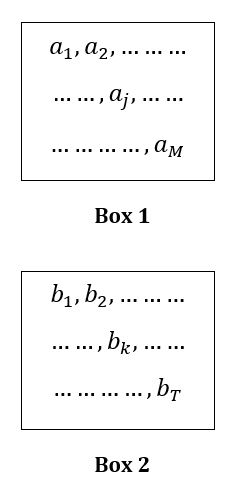
\includegraphics[width=4.5cm, height= 8cm]{SS figures/SS2.JPG}
\caption{Two Boxes}\label{SS2}
\end{wrapfigure}

Suppose $y$ denotes amounts gained or lost last last week in gambling or spent in giving wine-parties last year  or income taxes evaded or numbers of induced abortions  experienced so far etc. A person labelled $i$ and selected no matter how may be approached with $2$ boxes respectively containing similar cards marked $\{a_1, \cdots , a_j, \cdots, a_M\}$ in the first and $\{b_1,\cdots,b_k,\cdots,b_T\}$ in the second with means and variances respectively as known as 
\begin{align*}
    \mu_A & = \dfrac{1}{M}\sum_{j=1}^M a_j , \quad \sigma_A^2 = \dfrac{1}{M}\sum_{j=1}^M (a_j-\mu_A)^2 \\
    \text{and}\quad \mu_B & = \dfrac{1}{T}\sum_{k=1}^T b_k , \quad \sigma_B^2 = \dfrac{1}{T}\sum_{k=1}^T (b_k -\mu_B)^2.
\end{align*}

Then the selected person labelled $i$ is requested to draw one card marked, say, $a_j$, from the $1^{st}$ box and then independently from the $2^{nd}$ box to draw one card, say, marked as $b_k$, and report the randomized number as, say, $$z_i = a_jy_i + b_k$$ to the interviewer. The interviewer will not notice the values $a_j,\ b_k $ and $y_i$, nothing, will just receive the value $z_i$ from the $i^{th}$ selected respondent. Thus the privacy of the respondent is protected. Then,
\begin{align*}
  \E_R(z_i)  & = \E_R(a_jy_i + b_k)  \\
  & = y_i \E_R(a_j) +\E_R(b_k), \ [\text{Note that, once a respondent is selected in sample, his $y_i$ value is fixed.}]\\
  & = y_i\mu_A + \mu_B
\end{align*}
Hence, if $r_i = \dfrac{z_i-\mu_B}{\mu_A}$, assuming $\mu_A\neq 0$, then,
$$\E_R(r_i)=y_i .$$
Also, note that,
\begin{align*}
    \Var_R(r_i) & = \dfrac{\Var_R(z_i)}{\mu_A^2}=\dfrac{\sigma_A^2y_i^2 + \sigma_B^2}{\mu_A^2}\\
    \text{i.e,}\quad \Var_R(r_i) & = y_i^2\dfrac{\sigma_A^2}{\mu_A^2} + \dfrac{\sigma_B^2}{\mu_A^2}\\
    & = \alpha y_i^2 + \beta , \quad \text{(say)}.
\end{align*}
Now to obtain an unbiased estimator of $\Var_R(r_i)$, let us proceed as follows.

Let us start with $\alpha r_i^2 +\beta $. Then,
\begin{align*}
    \E_R(\alpha r_i^2 +\beta) & = \alpha \E_R(r_i^2)+\beta \\
    & = \alpha\left\{\Var_R(r_i) + (\E_R(r_i))^2\right\}+\beta \\
    & = \alpha \Var_R(r_i) +\alpha y_i^2 +\beta \\
    & = \alpha \Var_R(r_i) + \Var_R(r_i) \\
    & = (1+\alpha)\Var_R(r_i)\\
    \implies \Var_R(r_i) & = \E_R\left(\dfrac{\alpha r_i^2 +\beta}{1+\alpha}\right)\\
    \implies \hat{\Var}_i = \hat{\Var}_R(r_i) & = \dfrac{\alpha r_i^2 +\beta}{1+\alpha} .
\end{align*}

So now taking $e =\displaystyle\sum_{i=1}^N b_{si}I_{si}r_i$, we have,
\begin{align*}
    \E_P\E_R(e) & = \E_P\E_R\left(\sum_{i=1}^N b_{si}I_{si}r_i\right)\\
    & = \E_P\left(\sum_{i=1}^N b_{si}I_{si}\E_R(r_i)\right)\\
    & = \E_P\left(\sum_{i=1}^N b_{si}I_{si}y_i\right)\\
    & = \E_P(t(s,\mathbf{y}))\\
    & = Y
\end{align*}
Hence, $e=\displaystyle\sum_{i=1}^N b_{si}I_{si}r_i$ can be taken as an unbiased estimator of $Y$ and its variance estimator can be taken as,
$$\hat{\Var}(e)=\left.v_P(t)\right|_{\mathbf{y}=\mathbf{R}}+\sum_{i\in s} \hat{\Var}_i (b_{si}^2-d_{si}).$$

\subsection{Some Other Improvements in RR Models}

In Warner (1965)'s technique the attribute $A$ and its complement $A^c$ may both be stigmatizing like ``being Pro-Communist" and ``being Anti-Communist". As a consequence a respondent may feel uncomfortable to say ``YES" as also to say ``NO" or to say ``Match" as also to say ``No-Match" to a query implying $I_i$ either to be $1$ or $0$ for an $i^{th}$ labelled person. An alternative technique avoiding the difficulty developed by Greenberg et al. (1969) is as follows:-----

\begin{wrapfigure}{r}{7.5cm}
\centering
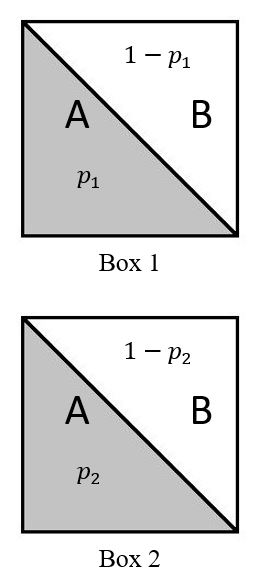
\includegraphics[width=4cm, height= 8cm]{SS figures/SS3.JPG}
\caption{2 Boxes}\label{SS3}
\end{wrapfigure}

A person labelled $i$, no matter how selected, is approached by the investigator carrying $2$ boxes, namely Box $1$ and Box $2$.

Box $1$ contains  cards marked $A$ and $B$ in proportions $p_1:(1-p_1)$ and Box $2$ contains  cards marked $A$ and $B$ in proportions $p_2:(1-p_2)$, $p_1 \neq p_2$.

Here note that, $A$ represents the sensitive attribute and $B$ represents an another non-sensitive attribute completely unrelated to the sensitive attribute $A$.
 
 The selected respondent is asked to draw one card each from $2$ boxes independently and returned to it after responding
 $$I_i=\begin{cases}
 1 & \text{if card from $1^{st}$ box ``matches" with the}\\
  & \text{actual trait of the respondent,}\\
  0 & \text{if ``No Match",}
 \end{cases}$$
$$J_i=\begin{cases}
 1 & \text{if card from $2^{nd}$ box ``matches" with the}\\
  & \text{actual trait of the respondent,}\\
  0 & \text{if ``No Match".}
 \end{cases}$$
Note the $B$ attribute can be considered as ``Do you prefer cricket to football ?" or ``Does your birthday fall in between January and June ?" or something like these. Hence the attribute $B$ is called completely unrelated with the actual sensitive characteristics $A$.

Hence,
$$\E_R(I_i)=p_1y_i+(1-p_1)x_i,$$
considering,
$$x_i = \begin{cases}
1 & \text{if $i^{th}$ person has unrelated trait $B$,}\\
0 & \text{otherwise.}
\end{cases}$$
Similarly,
$$\E_R(J_i)=p_2y_i+(1-p_2)x_i.$$
So, we can have
$$\E_R[(1-p_2)I_i-(1-p_1)J_i]=(p_1-p_2)y_i.$$
Hence if we call $r_i=\dfrac{(1-p_2)I_i-(1-p_1)J_i}{p_1-p_2}$, provided $p_1 \neq p_2$, we have 
$$\E_R(r_i)=y_i$$
and
$$\Var_R(r_i)=\dfrac{(1-p_2)^2 \Var_R(I_i)-(1-p_1)^2 \Var_R( J_i)}{(p_1-p_2)^2}.$$
Now, 
\begin{align*}
   \Var_R(I_i) & = \E_R(I_i^2) - (\E_R(I_i))^2\\
   & = \E_R(I_i)-(\E_R(I_i))^2 \quad [\because I_i=0\ \text{or}\ 1 \implies I_i^2=I_i]
\end{align*}
and similarly,
$$\Var_R(J_i)= \E_R(J_i)-(\E_R(J_i))^2\quad [\because J_i=0\ \text{or}\ 1 \implies J_i^2=J_i].$$
Now to estimate $\Var_R(r_i)$, we note that,
\begin{align*}
    \Var_R(r_i) & = \E_R(r_i^2) - (\E_R(r_i))^2\\
    & = \E_R(r_i^2)-y_i^2\\
    & = \E_R(r_i^2)-y_i, \quad \text{as}\quad  y_i=0\ \text{or}\ 1, \\
    & = \E_R(r_i^2)-\E_R(r_i)
\end{align*}
Hence, $\Var_R(r_i)=\E_R(r_i^2-r_i)= \E_R[r_i(r_i-1)]$. That means, $\hat{\Var}_i=r_i(r_i-1)$ satisfies 
$$\E_R\left(\hat{\Var}_i\right)=\Var_i=\Var_R(r_i).$$
So, estimates of $Y$ and then of $\theta=\dfrac{Y}{N}$ and variance estimators can be produced as before.

\subsection{Practical Illustrations}

For example, if one implies a sampling scheme that permits $\pi_i > 0\ \forall i \in U = \{1,2,\cdots,N\}$ and $\pi_{ij}>0$ for $i\neq j \in U = \{1,2,\cdots,N\}$, and applies a RR model having $r_i$ as modified responses that have $\E_R(r_i)=y_i$ and $\Var_R(r_i)$ is unbiased estimator $\hat{\Var}_i$, then an unbiased estimator for sensitive population mean or proportions can be taken as $\dfrac{e}{N}=\dfrac{1}{N}\sum_{i \in s}\dfrac{r_i}{\pi_i}$ with unbiased variance estimator as,
\begin{align*}
    v\left(\dfrac{e}{N}\right)& = \dfrac{1}{N^2}v(e)\\
    & =\dfrac{1}{N^2} \left[\left.v_P(t)\right|_{\mathbf{y}=\mathbf{R}}+\sum_{i\in s} (b_{si}^2-d_{si})\hat{\Var}_i \right],\quad \text{where}\  t=\sum_{i \in s}\dfrac{y_i}{\pi_i},
\end{align*}
Recall that,
\begin{align*}
    \Var_P\left(t_{HT}=\sum_{i \in s}\dfrac{y_i}{\pi_i}\right) & = \E_P\left(\sum_{i \in s}\dfrac{y_i}{\pi_i}\right)^2-\left(\E_P\left(\sum_{i \in s}\dfrac{y_i}{\pi_i}\right)\right)^2\\
    & = \E_P\left(\sum_{i \in s}\dfrac{y_i^2}{\pi_i^2}+\sum_{i \in s}\sum_{\substack{j\in s \\ j\neq i}}\dfrac{y_iy_j}{\pi_i\pi_j}\right)-Y^2\\
    & = \E_P\left(\sum_{i \in s}\dfrac{y_i^2}{\pi_i}\cdot \dfrac{1}{\pi_i}\right)+\E_P\left(\sum_{i \in s}\sum_{\substack{j\in s \\ j\neq i}}\dfrac{y_iy_j}{\pi_i\pi_j}\right)-Y^2\\
    & = \sum_{i=1}^N \dfrac{Y_i^2}{\pi_i}+ \sum_{s \in \mathcal{S}}p(s)\left(\sum_{i \in s}\sum_{\substack{j\in s \\ j\neq i}}\dfrac{y_iy_j}{\pi_i\pi_j}\right)-Y^2 \\
    & = \sum_{i=1}^N \dfrac{Y_i^2}{\pi_i} + \sum_{i=1}^N\sum_{j\neq i}^N\dfrac{Y_iY_j}{\pi_i\pi_j}\sum_{s \contains i,j} p(s) -Y^2\\
    & = \sum_{i=1}^N \dfrac{Y_i^2}{\pi_i} + \sum_{i=1}^N\sum_{j\neq i}^N\dfrac{Y_iY_j}{\pi_i\pi_j}\pi_{ij} - Y^2\\
    & = \sum_{i=1}^N \dfrac{Y_i^2}{\pi_i} + \sum_{i=1}^N\sum_{j\neq i}^N\dfrac{Y_iY_j}{\pi_i\pi_j}\pi_{ij} - \sum_{i=1}^N Y_i^2 - \sum_{i=1}^N\sum_{j\neq i}^N Y_i Y_j \\
    & = \sum_{i=1}^N Y_i^2 \left(\dfrac{1-\pi_i}{\pi_i}\right) + \sum_{i=1}^N\sum_{j\neq i}^N Y_i Y_j \left(\dfrac{\pi_{ij}-\pi_i\pi_j}{\pi_i\pi_j}\right)
\end{align*}
Hence, $b_{si}=\dfrac{1}{\pi_i},\ d_i = \dfrac{1-\pi_i}{\pi_i},\ d_{ij}= \dfrac{\pi_{ij}-\pi_i\pi_j}{\pi_i\pi_j}$. So, $d_{si}$ and $d_{sij}$'s are given by,
$$d_{si}=\dfrac{1-\pi_i}{\pi_i^2},\quad d_{sij}= \dfrac{\pi_{ij}-\pi_i\pi_j}{\pi_i\pi_j\pi_{ij}},$$
because $\E_P(d_{si}I_{si})=d_i$ and $\E_P(d_{sij}I_{sij})=d_{ij}$.

So, 
\begin{align*}
    v_P(t) & =\sum_{i \in s} y_i^2d_{si} +\displaystyle \sum_{i \in s}\sum_{\substack{j\in s \\ j\neq i}}
    y_iy_jd_{sij}\\
    & = \sum_{i \in s} y_i^2 \left(\dfrac{1-\pi_i}{\pi_i^2}\right) + \sum_{i \in s}\sum_{\substack{j\in s \\ j\neq i}} y_iy_j\left(\dfrac{\pi_{ij}-\pi_i\pi_j}{\pi_i\pi_j\pi_{ij}}\right)
\end{align*}
Hence,
\begin{align*}
    v(e) & = \left.v_P(t)\right|_{\mathbf{y}=\mathbf{R}}+\sum_{i\in s} (b_{si}^2-d_{si})\hat{\Var}_i \\
    & = \sum_{i \in s} r_i^2 \left(\dfrac{1-\pi_i}{\pi_i^2}\right) + \sum_{i \in s}\sum_{\substack{j\in s \\ j\neq i}} r_ir_j\left(\dfrac{\pi_{ij}-\pi_i\pi_j}{\pi_i\pi_j\pi_{ij}}\right) + \sum_{i\in s} \left(\dfrac{1}{\pi_i^2}-\dfrac{1-\pi_i}{\pi_i^2}\right)\hat{\Var}_i \\
    & = \sum_{i \in s} r_i^2 \left(\dfrac{1-\pi_i}{\pi_i^2}\right) + \sum_{i \in s}\sum_{\substack{j\in s \\ j\neq i}} r_ir_j\left(\dfrac{\pi_{ij}-\pi_i\pi_j}{\pi_i\pi_j\pi_{ij}}\right) + \sum_{i\in s} \dfrac{\hat{\Var}_i}{\pi_i}.
\end{align*}


%%%%% CLASS 7

\subsection{Protections of Privacy}

At the initial stage, Warner (1965) and other statisticians developed the theory of estimated of the proportions $\theta$, with $0 < \theta < 1$, of people bearing a sensitive characteristic $A$ and the allied variance estimation problems based on sample selection of respondents using SRSWR scheme and rarely through SRSWOR scheme at most. But not through the general sampling schemes with unequal probabilities, the problem was considered.

In choosing an SRSWR of $n$ draws, the probability that a person bears characteristic $A$ is $\theta$, and this is so at every draw. For Warner's (1965) model and some other models, the RR's gathered area "Yes i.e. Match" or "No i.e. Non-Match". 

Now, we have $\prob(A) = 0$ and $\prob(A^c) = (1-\theta)$. Let, $\prob(\text{Yes} \mid A) = a$ and $\prob(\text{No} \mid A^c) = b$. Then, by use of Bayes' theorem, as noted by Nayak (1994),

\begin{align*}
    \prob(A \mid \text{Yes}) 
    & = \dfrac{\prob(A) \prob(\text{Yes}\mid A) }{\prob(A) \prob(\text{Yes}\mid A) + \prob(A^c) \prob(\text{Yes}\mid A^c)}\\
    & = \dfrac{\theta a}{\theta a + (1-\theta) (1-b)}
\end{align*}

If $\prob(A \mid \text{Yes}) > \prob(A)$, then a person may hesitate to give a "yes" response because he / she may perceive this response to enhance his / her being inferred to bear $A$ rather than $A^c$.

Similarly,

\begin{align*}
    \prob(A^c \mid \text{No}) 
    & = \dfrac{\prob(A^c) \prob(\text{No}\mid A^c) }{\prob(A) \prob(\text{No}\mid A) + \prob(A^c) \prob(\text{No}\mid A^c)}\\
    & = \dfrac{(1 - \theta) b}{\theta (1-a) + (1-\theta) b}
\end{align*}

Now if $\prob(A^c \mid \text{No}) < (1-\theta)$, then "No" answer may appear jeopardizing to a respondent's privacy.

\begin{definition}
    So, for a response $R$ as either "Yes" or "No", the quantity,
    $$J(R) = \dfrac{\prob(A\mid R)/\theta}{\prob(A^c \mid R)/(1-\theta)}$$
    is taken as a \textbf{Measure of Jeopardy} in pronouncing a RR as R("Yes or "No") by a respondent, where $\prob(A\mid R)$ and $\prob(A^c\mid R)$ are probabilities of "revealing" one's true feature being $A$ or $A^c$, conditional on their response $R$.
\end{definition}

The ideal value of $J(R)$, whether $R$ is "Yes" or "No", which protects a respondent's identity is unity. The father it is away from unity the less the response $R$ protects one's privacy.

For Warner's (1965) scheme, 

\begin{align*}
    \prob(A \mid \text{Yes}) 
    & = \dfrac{\prob(A) \prob(\text{Yes}\mid A) }{ \prob(A) \prob(\text{Yes}\mid A) + \prob(A^c) \prob(\text{Yes}\mid A^c) }\\
    & = \dfrac{\theta p}{\theta p + (1-\theta) (1-p)}\\
    & = \dfrac{\theta p}{ \theta p + (1 - \theta) - p + \theta p }\\
    & = \dfrac{\theta p}{(1 - p) + (2p - 1)\theta}
\end{align*}

when $p = 1/2$, and $\prob(A \mid \text{Yes}) = \theta$.

But we know that in Warner's (1965) RRD, $p = 1/2$ is not permissible. And also variance of the estimator $\rightarrow \infty$ and $\vert p - 1/2 \vert \rightarrow 0$. So, we see that a respondent's privacy can be protected at the cost of huge loss in efficiency in estimation in Warner's RR model.

For other RR techniques also it is possible to check that "as the privacy is protected more and more" the efficiency in estimation simultaneously goes on declining.

\subsection{Protection of Privacy for General Sampling Design with Unequal probabilities with or without replacement}

Note that in choosing an SRSWR of $n$ draws, the probability that a person bears the sensitive characteristic $A$ is $\theta$ and this is so for every draw. But, for general sampling scheme with unequal probability, this probability does not remain same at every draw. For this reason, the protection of privacy for general sampling design is to be studied in some different way.

Chaudhuri, Christofides and Saha (2008) have a generalized measure of jeopardy defined for RR's based on some specific RRT's for general sampling designs with unequal probabilities with or without replacement. Bayesian approach is utilized for this purpose. A prior probability distribution is postulated for the response qualitative sensitive variable $y$ which takes a value either $1$ or $0$.

Let, $L_i (0 < L_i < 1)$ be the probability that $y_i$ takes the value $1$ i.e. $L_i = \prob(y_i = 1)$.

Let, $L_i(R)$ denote the conditional probability that $i$-th respondent bears $A$ given that his / her randomized response is $R$. Then,

$$J_i(R) = \dfrac{L_i(R) / L_i}{(1 - L_i(R)) / (1 - L_i) } \quad i \in U$$

is defined as the \textbf{Response specific Jeopardy measure} for the RR gathered as $R$ from the person labelled $i$.

Let us now write $1$ for RR $R$ as "Yes i.e. Match" and $0$ for RR $R$ as "No i.e. non-match". Now note that, $1$ or $0$ are the only possible values of $R$.  Considering these two only possible values of $R$, for a respondent labelled $i$, the average Jeopardy measure is defined as;

$$\overline{J_i} = \dfrac{1}{2} \left( J_i(1) + J_i(0) \right)$$

An ideal value of $\overline{J_i}$ is unity, ensuring the maximal privacy protection for respondent $i$.

Let us now see how this approach can be used. For Warner's RRT, irrespective of how a person $i$ is sampled,

\begin{align*}
    L_i(1) 
    & = \text{Conditional probability that person } i \text{ bears } A\\
    & \qquad \text{given that his RR is 1 i.e. "Yes" i.e. "Match"}\\
    & = \dfrac{\prob(\text{Person } i \text{ bears } A \text{ and his RR is 1})}{\prob(\text{Person } i \text{has his RR equal to 1})}\\
    & = \dfrac{L_i \prob(I_i = 1 \mid y_i = 1)}{L_i \prob(I_i = 1 \mid y_i = 1) + (1 - L_i) \prob(I_i = 1 \mid y_i = 0) }\\
    & = \dfrac{L_i p}{L_i p + (1-L_i) (1 - p)}\\
    & = \dfrac{pL_i}{(1 - p) + (2p - 1)L_i}
\end{align*}

Similarly, 

\begin{align*}
    L_i(0)
    & = \dfrac{L_i \prob(I_i = 0 \mid y_i = 1)}{L_i \prob(I_i = 0 \mid y_i = 1) + (1 - L_i) \prob(I_i = 0 \mid y_i = 0)}\\
    & = \dfrac{L_i (1-p)}{L_i (1-p) + (1-L_i) p}\\
    & = \dfrac{L_i(1-p)}{p + (1-2p)L_i}
\end{align*}

Note that, as $p \rightarrow \frac{1}{2}$, both $L_i(1)$ and $L_i(0) \rightarrow L_i$, but $\Var_i = \Var_R(r_i) = \dfrac{p(1-p)}{(1-2p)^2} \rightarrow \infty$.

Also, we have the following theorem.

\begin{theorem}
    The Jeopardy measures $J_i(1)$ and $J_i(0)$ are independent of the values $L_i$, rather is the odds ratio based on the proportion $p$.
\end{theorem}

\begin{proof}
    Note that,
    \begin{align*}
        J_i(1)
        & = \dfrac{L_i(1)/L_i}{(1 - L_i(1)) / (1 - L_i)}\\
        & = \dfrac{p / \left[ (1-p) + (2p-1)L_i \right]}{ \left[ 1 - \dfrac{pL_i}{(1-p) + (2p-1)L_i}\right] / (1 - L_i)}\\
        & = \dfrac{p(1-L_i) \left( (1-p) + (2p-1)L_i \right) }{ \left( (1-p) + (2p-1)L_i \right) \left( (1-p) + (2p-1)L_i - pL_i \right) }\\
        & = \dfrac{p(1- L_i)}{ (1-p) + 2pL_i - L_i - pL_i }\\
        & = \dfrac{p(1- L_i)}{ (1-p) - L_i(1-p) }\\
        & = \dfrac{p (1- L_i)}{(1 - p) (1 - L_i)} = \dfrac{p}{(1-p)}
    \end{align*}

    In a very similar way,
    \begin{align*}
        J_i(0)
        & = \dfrac{L_i(0)/L_i}{(1 - L_i(0)) / (1 - L_i)}\\
        & = \dfrac{(1-p) / \left[ p + (1 - 2p)L_i \right]}{ \left[ 1 - \dfrac{(1-p)L_i}{p + (1 - 2p)L_i}\right] / (1 - L_i)}\\
        & = \dfrac{(1-p)(1-L_i)}{p + (1-2p)L_i - (1-p)L_i}\\
        & = \dfrac{(1-p)}{p}
    \end{align*}
\end{proof}

\begin{corollary}
    Hence, $\overline{J_i} = \dfrac{1}{2}\left( \dfrac{(1-p)}{p} + \dfrac{p}{(1-p)} \right)$. Clearly, this tends to the value of unity only when $p \rightarrow \dfrac{1}{2}$, and hence $\Var_i \rightarrow \infty$. This means, privacy protection can be increased here only at the cost of losing efficiency.
\end{corollary}




%%%%%%% class 8

\section{Sampling Strategy for hadling Non Response Bias}

\subsection{Pollitz and Simmons at home technique to handle non response}

We have studied earlier Hansen and Hurwitz's re-attempt technique to handle non responses by Double sampling approach.

In the cases where the cost of collection information at the re-attempt is far higher than that based on the first attempt, Pollitz and Simmons (1949, 1950, JASA) have introducted the method of using the probabilities at-home to estimate the population mean of a variable of interest. It is used when the major casue of non interviews is the absence of respondents at home when the interviewer knocks at the door. The interviewer makes only one call at each sampled household, the time of call being random within the interviewing hours. If the eligible respondent is available at the house, the desired information was collected and it is also asked whether the respondent was at home on the previous six days at the same time. This information is used to estimate $p$, the probability of being at home.

If the respondent is found to be away from home, no information is collected.

Assume that, an SRSWR of $n$ households are selected. Then from the data obtained corresponding to the $i$-th selected household we can have an estimate of $y_i$ as 

$$\widehat{y_i} = \begin{cases}
    \dfrac{y_i}{\widehat{p_i}} & \text{if the household is available}\\
    0 & \text{ otherwise}
\end{cases}
$$

where $\widehat{p_i}$ is an estimate of $p_i$, the probability of being at home of the $i$-th household. This $p_i$ can be estimated from the number of availablities out of $7$ days, (six days before and the interviewing date) by $\widehat{p_i} = j/s = j/7$, where $j$ is $1, 2, \dots 7 (=s)$, conditional on the consideration that at the time of interview, the household is available.

Hence, for a specified unit, the expected value of $\widehat{y_i}$ would be (given availability);

\begin{align*}
    \E(\widehat{y_i})
    & = \sum_{j = 1}^{s} \dfrac{y_i}{j/s} \binom{s-1}{j-1} p_i^{j-1} (1 - p_i)^{s-j}\\
    & = y_i \sum_{j = 1}^{s} \dfrac{s}{j} \binom{s-1}{j-1} p_i^{j-1} (1 - p_i)^{s-j}\\
    & = y_i \sum_{j = 1}^{s} \binom{s}{j} p_i^{j-1} (1 - p_i)^{s-j}\\
    & = \dfrac{y_i}{p_i} \left[ 1 - q_i^s \right]
\end{align*}

where $q_i = (1 - p_i)$. So now, taking into account that the probability of availability of household $i$ is $p_i$ and Probability of selecting that household is $1/N$, the expectation becomes;

\begin{align*}
    \E(\widehat{y_i})
    & = \sum_{i = 1}^{N} \dfrac{Y_i (1 - q_i^s)}{p_i} \times p_i \times \dfrac{1}{N}\\
    & = \dfrac{1}{N} \sum_{i = 1}^{N} \left( Y_i - Y_i q_i^s \right)\\
    & = \overline{Y} - \dfrac{1}{N} \sum_{i=1}^{N} Y_i q_i^s
\end{align*}

\begin{theorem}
    The estimator $\widehat{\overline{Y_{PS}}} = \dfrac{1}{n}\sum_{i=1}^{n} \widehat{y_i}$ as our estimator for $\overline{Y}$, is not unbiased, and the bias is $- \dfrac{1}{N} \sum_{i=1}^{N} Y_i q_i^s$, which is very small as $q_i^s$ is small if $s$ is made sufficiently large.
\end{theorem}

Similar to the simple SRSWR variance estimator, we also have the following:

\begin{theorem}
    $$\widehat{\Var}\left( \widehat{\overline{Y_{PS}}} \right) = \dfrac{1}{n(n-1)} \sum_{i=1}^{n} \left( \widehat{y_i} - \dfrac{1}{n}\sum_{i=1}^{n}\widehat{y_i} \right)^2$$
\end{theorem}


\subsection{Other Approaches to handle non response}

Many other alternative approaches to handle incidence of Non responses are available in the literature. One of them is to estimate the probability of giving responses with the help of some suitable model postulation. Let us now discuss that.

Suppose from a survey population $U = \left\{1, 2, \dots i, \dots N \right\}$, a suitably large sample $s$ of size $n$ has been drawn with a probability $p(s)$ yielding inclusion probabilities $\pi_i$ for unit $i$ and $\pi_{ij}$ for pair of distinct units $i\neq j  = 1, 2, \dots N$. We can then employ Horvitz and Thompson's estimator, $t_{HT} = \sum_{i \in s} \dfrac{y_i}{\pi_i}$ for $Y = \sum_{i = 1}^{N} Y_i$.

But suppose the responses are available from a sub-sample $r$ of respondents in $s$, and the complementary set $m$ giving us the set of no responses.

Let, $q_i$ denote the unknown probability before the start of the survey that the $i$-th person will respond. Then,

$$e_{HT} = \sum_{i \in s} \dfrac{y_i}{\pi_i q_i} = \sum_{i \in s} \dfrac{e_i}{\pi_i}$$

on writing $e_i = y_i/q_i$, which might be taken as an unbiased estimator of $Y$ if $q_i$'s were known.

Let us define the indicator variables;

$$I_{si} = \begin{cases}
    1 & i \in s\\
    0 & i \notin s
\end{cases}$$

and 

$$I_{ri} = \begin{cases}
    1 & \text{if person } i \text{ in } s \text{ responds}\\
    0 & \text{if person } i \text{ in } s \text{ does not respond}
\end{cases}$$

Then, writing $\E_r, \Var_r$ as the expectation and variance operators with respect to the incidence of a sampled person's act of responding and $\E_p, \Var_p$ as the expectation and variance operators with respect to the selection in the sample according to the design $p$ and $\E, \Var$ denoting the overall expectation and variance operators, we have;

\begin{align*}
    \E & = \E_p \E_r\\
    \Var & = \E_p \Var_r + \Var_p \E_r
\end{align*}


Then,

\begin{align*}
    \E(e_{HT})
    & = \E\left( \sum_{i=1}^{N} Y_i \dfrac{I_{si}}{\pi_i} \dfrac{I_{ri}}{q_i} \right)\\
    & = \E_p \E_r\left( \sum_{i=1}^{N} Y_i \dfrac{I_{si}}{\pi_i} \dfrac{I_{ri}}{q_i} \right)\\
    & = \E_p \left( \sum_{i=1}^{N} Y_i \dfrac{I_{si}}{\pi_i} \dfrac{\E_r(I_{ri}) }{q_i} \right)\\
    & = \E_p\left( \sum_{i=1}^{N} Y_i \dfrac{I_{si}}{\pi_i} \dfrac{q_i}{q_i} \right)\\
    & = \E_p\left( \sum_{i=1}^{N} Y_i \dfrac{I_{si}}{\pi_i} \right)\\
    & = Y, \qquad \text{due to unbiasedness of Horvitz and Thompson's estimator}
\end{align*}

On the other hand,

\begin{align*}
    \Var(e_{HT})
    & = \Var\left( \sum_{i=1}^{N} Y_i \dfrac{I_{si}}{\pi_i} \dfrac{I_{ri}}{q_i} \right)\\
    & = \Var_p\E_r\left( \sum_{i=1}^{N} Y_i \dfrac{I_{si}}{\pi_i} \dfrac{I_{ri}}{q_i} \right) + \E_p \Var_r\left( \sum_{i=1}^{N} Y_i \dfrac{I_{si}}{\pi} \dfrac{I_{ri}}{q_i} \right)\\
    & = \Var_p\left( \sum_{i=1}^{N} Y_i \dfrac{I_{si}}{\pi_i} \right) + \E_p\left[ \sum_{i=1}^{N} Y_i^2 \dfrac{I_{si}^2}{\pi_i^2} \dfrac{\Var_r(I_{ri})}{q_i^2} \right]\\
    & = \Var_p\left( \sum_{i=1}^{N} Y_i \dfrac{I_{si}}{\pi_i} \right) + \E_p\left[ \sum_{i=1}^{N} Y_i^2 \dfrac{I_{si}^2}{\pi_i^2} \dfrac{q_i(1-q_i)}{q_i^2} \right]\\
    & = \sum_{i=1}^{N} Y_i^2 \dfrac{(1 - \pi_i)}{\pi_i} + \sum_{i\neq j}^{N} Y_i Y_j (\pi_{ij} - \pi_i \pi_j) + \E_p\left[ \sum_{i=1}^{N} \left(Y_i^2\dfrac{(1-q_i)}{\pi_i q_i}\right) \dfrac{I_{si}}{\pi_i}  \right]\\
    & = \sum_{i=1}^{N} Y_i^2 \dfrac{(1 - \pi_i)}{\pi_i} + \sum_{i\neq j}^{N} Y_i Y_j (\pi_{ij} - \pi_i \pi_j) + \sum_{i=1}^{N} \left(Y_i^2\dfrac{(1-q_i)}{\pi_i q_i}\right)\\
    & = \sum_{i=1}^{N} Y_i^2 c_i + \sum_{i \neq j}^{N} Y_iY_jc_{ij}
\end{align*}

where 

$$c_i = \dfrac{(1 - \pi_i)}{\pi_i} + \dfrac{(1-q_i)}{q_i \pi_i}$$

and 

$$c_{ij} = \pi_{ij} - \pi_i \pi_j$$

Thus, an unbiased estimator of this variance is;

$$\widehat{\Var}(e_{HT}) = v(e_{HT}) = \sum_{i=1}^{N} Y_i^2 c_i \dfrac{I_{si}}{\pi_i} \dfrac{I_{ri}}{q_i} + \sum_{i \neq j}^{N} Y_iY_jc_{ij} \dfrac{I_{s,ij}}{\pi_{ij}} \dfrac{\pi_{ri}}{q_i} \dfrac{\pi_{rj}}{q_j}$$

provided all $q_i$'s are known.

Since, $q_i$'s are not known, let us turn our attention to this aspect of the problem.

From past experiences and remarks obtained from the sampling expert entrusted with the survey under consideration, let $\widehat{q_i}$ be some priliminary guessed values or estimate of $q_i$ such that $0 < \widehat{q_i} < 1$. Consider the logit transformation on this $\widehat{q_i}$'s, namely, say $\widehat{r_i} = \log\left( \dfrac{\widehat{q_i}}{(1 - \widehat{q_i})} \right)$ and we consider the following model;

$$\widehat{r_i} = r_i + \epsilon_i, \qquad i \in U$$

where $r_i = \log\left( \dfrac{q_i}{(1 - q_i)} \right)$. Let us also consider that some variable $x_i \forall i \in U$, which is well correlated with the study variable $y$ is available.

Then,

$$\widehat{r_i} = r_i + \epsilon_i = \alpha + \beta x_i + \epsilon_i, \qquad i \in U$$

model may be considered, where $\epsilon_i$'s are random errors $\widehat{r_i} - r_i, i \in U$. By least squares principle, on minimizing $S = \sum (\hat{r_i} - \alpha - \beta x_i)^2$ with respect to $\alpha, \beta$, one may obtain the least squares estimates as;

\begin{align*}
    \widehat{\beta} & = \dfrac{\sum_{i \in s} \hat{r_i} (x_i - \bar{x}) }{ \sum_{i \in s} (x_i - \bar{x})^2 }\\
    \widehat{\alpha} & = \overline{\widehat{r}} - \widehat{\beta}\bar{x}
\end{align*}


These yield estimates of $r_i$ as $r_i^\ast = \widehat{\alpha} + \widehat{\beta}x_i, i \in U$. And hence the estimates of $q_i$ can be obtained by inverse logit transformation,

$$q_i^\ast = \dfrac{e^{\widehat{\alpha} + \widehat{\beta}x_i }}{1 + e^{\widehat{\alpha} + \widehat{\beta}x_i } }$$

Replacing $q_i$ in $e_{HT}$ and $v(e_{HT})$ by $q_i^\ast$ one may obtain a revised estimator $\widehat{e_{HT}}$ and $v(\widehat{e_{HT}})$, which can be used as an estimate and can be obtained completely from all the known information of the sample.

\end{document}